\begin{enumerate}[label=\thesection.\arabic*.,ref=\thesection.\theenumi]
\numberwithin{equation}{enumi}

\item For an LTI system, the Bode plot for its gain defined as
\begin{align}
	G(s) = 20\log\abs{H(s)}
	\label{eq:ee18btech11001_gain}
\end{align}
is as illustrated in the Fig. \ref{fig:ee18btech11001_bode}. Express $G(f)$ in terms of $f$.\\
\begin{figure}[ht!]
    \includegraphics[width=\columnwidth]{./figs/ee18btech11001/ee18btech11001.eps}
    \caption{}
    \label{fig:ee18btech11001_bode}
\end{figure}\\

\solution
\begin{align}
 G(f) = 
 \begin{cases} 
        100 & 0 < f < 10^{1} \\
      120-20\log(f) & 10 < f < 10^{2} \\
      200-60\log(f) & 10^2 < f < 10^{3} \\
      140-40\log(f) & 10^{3} < f < 10^{4} \\
       -20 & 10^{4} < f < 10^{5} \\
      180-40\log(f) & 10^{5} < f < 10^{6} \\
      300-60\log(f) & 10^{6} < f < 10^{7}   
 \end{cases}
\end{align}

%-----------------------------------------------------------------------%

\item Express the slope of $G(f)$ in terms of $f$.
\\
\solution The desired slope is 
\begin{align}
\nabla G(f) &= \dfrac{d(G(f))}{d(\log(f))}
\end{align}

\begin{align}
 \nabla G(f) = 
 \begin{cases} 
        0 & 0 < f < 10^{1} \\
      -20 & 10 < f < 10^{2} \\
      -60 & 10^{2} < f < 10^{3} \\
      -40 & 10^{3} < f < 10^{4} \\
       0 & 10^{4} < f < 10^{5} \\
      -40 & 10^{5} < f < 10^{6} \\
      -60 & 10^{6} < f < 10^{7}   
 \end{cases}
\end{align}

%-----------------------------------------------------------------------%

\item Express the change of slope of $G(f)$ in terms of $f$.
\\
\solution\\
$\Delta(\nabla G(f))$  = Change of slope G(f) at f

\begin{align}
 \Delta(\nabla G(f)) = 
 \begin{cases} 
      -20 &  f = 10^{1} \\
      -40 &  f = 10^{2} \\
      +20 &  f = 10^{3} \\
      +40 &  f = 10^{4} \\
      -40 &  f = 10^{5} \\
      -20 &  f = 10^{6} 
 \end{cases}
\label{eq:ee18btech11001_slope_diff}
\end{align}

%-----------------------------------------------------------------------%

\item Tabulate the poles and zeros of $H(s)$ using \eqref{eq:ee18btech11001_slope_diff}.
\\
\solution Table \ref{table:ee18btech11001} provides the details.  
%
\begin{table}[!ht]
\centering
\begin{enumerate}[label=\thesubsection.\arabic*.,ref=\thesubsection.\theenumi]
\numberwithin{equation}{enumi}
\item A position control system is to be designed such that maximum peak overshoot is less than 25 \%.
Further, appropriate error constant should be 50. For the motor to be used, load and torque
speed curve is shown below, where, $J_{1}$ = 2 kg-m2
, $J_{2}$ = 18 kg-m2
, $f_{1}$ = 2 N-m-s/rad, $f_{2}$ = 36 N-ms/rad. (Although obvious, consider position as the controlled variable and armature voltage as
the manipulated variable.). 
\begin{enumerate}[label=(\roman*)]
\item Design a lead compensator for the system.
\item Design a lag compensator for the system.
\end{enumerate}

\begin{figure}[!ht]
\centering
    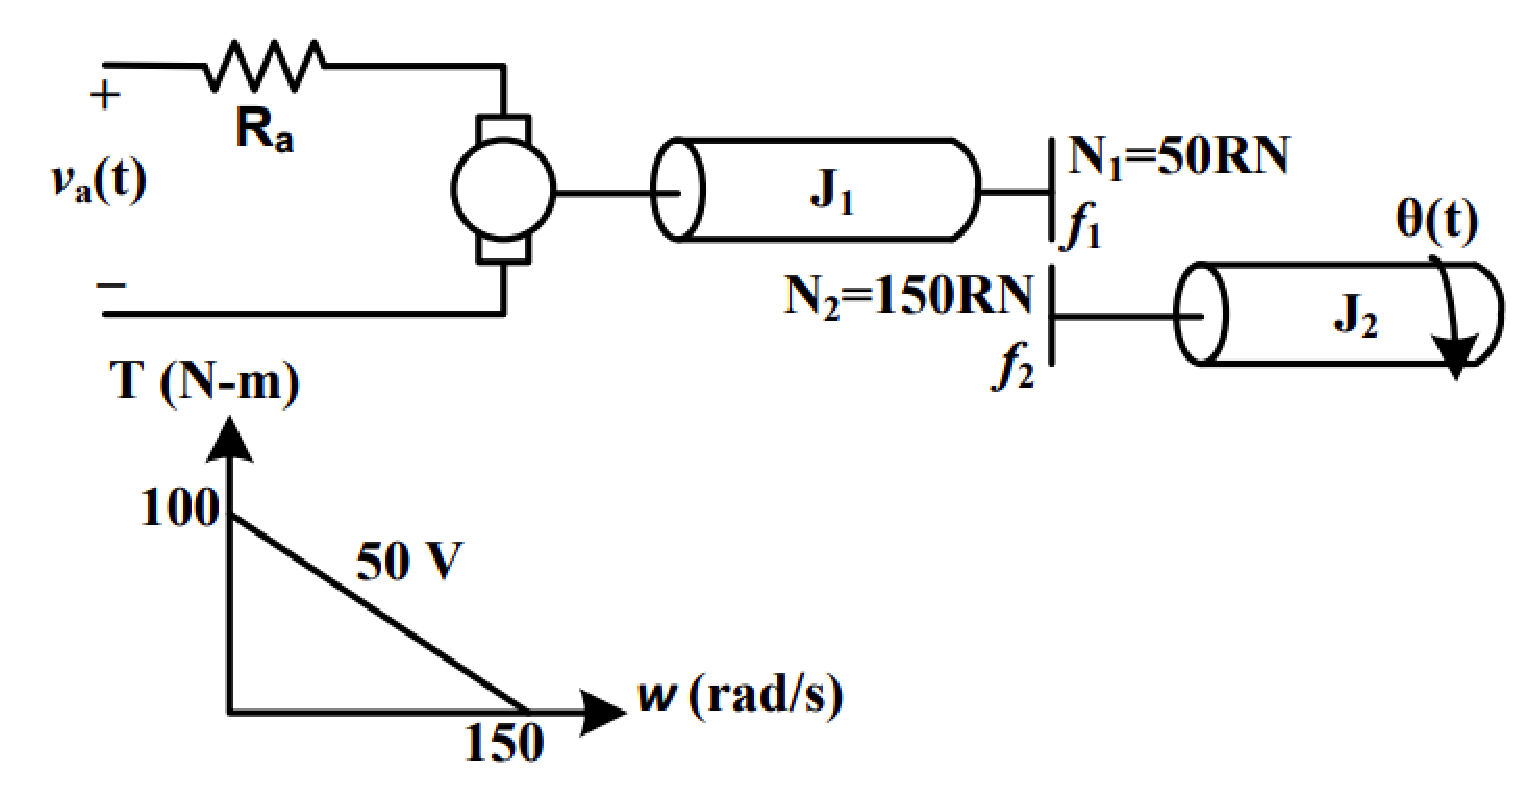
\includegraphics[width=\columnwidth]{./figs/ee18btech11001/ee18btech11001_1.eps}
  \caption{}
  \label{fig:ee18btech11001_fig1}
\end{figure}
%
\solution
Solving the system shown in \ref{fig:ee18btech11001_fig1},

From speed-torque curve of DC Motor in figure. Let $\vec{T_{m}}$ be the torque exerted by DC Motor.  \ref{fig:ee18btech11001_fig1}
\begin{align}
   \vec{T_{m}} &=  \frac{\vec{K_{T}}}{R_{a}}V_{a} - \frac{\vec{K_{T}}.\vec{K_{v}^{T}}}{R_{a}}\bm{\omega_{1}}
   \\
   \vec{T_{m}} &=  2V_{a} - \frac{2}{3}\bm{\omega_{1}}
    \label{eq:ee18btech11001_1}
\end{align}

\begin{table}[!ht]
\centering
\input{./tables/ee18btech11001_3.tex}
\caption{List of Variables}
\label{table:ee18btech11001_3}
\end{table}
Change in torque across ends = torque applied on load + viscous friction. On $J_{1}$ at one end torque $T_{m}$ is applied and at the other end $T_{1}$ exists.
\begin{align}
    \vec{T_{m}} &= \vec{T_{1}} + J_{1}\bm{\Ddot{\theta_{1}}} + f_{1}\bm{\Dot{\theta_{1}}} 
    \label{eq:ee18btech11001_2}
\end{align}
Similarly for $J_{2}$
\begin{align}
    \vec{T_{2}} &=  J_{2}\bm{\Ddot{\theta_{2}}} + f_{2}\bm{\Dot{\theta_{2}}} 
    \label{eq:ee18btech11001_3}
    \\
    \vec{T_{2}} &= \frac{N_{2}}{N_{1}} \vec{T_{1}} \text{ (Gear Train Formula)} \label{eq:ee18btech11001_4}
    \\
    \bm{\theta_{2}} &= \frac{N_{1}}{N_{2}} \bm{\theta_{1}} \text{ (Gear Train Formula)} \label{eq:ee18btech11001_5}
\end{align}

\begin{table}[!ht]
\centering
\input{./tables/ee18btech11001_4.tex}
\caption{Vectors and Matrices}
\label{table:ee18btech11001_4}
\end{table}    
Converting to State Space model
\begin{align}
    \bm{\theta} &= \myvec{\bm{\theta_{1}} \\ \bm{\theta_{2}}}
    \\
    3 \Vec{T_{m}} &= \myvec{3J_{1} & J_{2}}\bm{\Ddot{\theta}}+ \myvec{3f_{1} & f_{2}}\bm{\dot{\theta}}
    \\
    \Vec{T_{m}} &= 2V_{a} - \myvec{\frac{2}{3} & 0}\bm{\dot{\theta}}
    \\
    \bm{\theta} &= \myvec{N_{2} & 0 \\ 0& N_{1}} K
\end{align}
This is the state space model obtained
\begin{align}
    \bm{\Ddot{\theta}} &= \myvec{\frac{-13}{6} & 0 \\ 0 &\frac{-5}{3}}\bm{\Dot{\theta}} + \myvec{\frac{1}{2} \\ \frac{1}{6}}V_{a}
    \\
    \bm{\dot{\theta_{2}}} &= \myvec{0 \\ 1}\bm{\dot{\theta}} 
\end{align}
On solving the above State Space Model
\begin{align}
    V_{a}(s) &= (6s+10)(s\theta_{2}(s)) \label{eq:ee18btech11001_6}
    \\
    G(s) &=  K \frac{\theta (s)}{V_{a}(s)} = \frac{K}{2s(3s+5)} \label{eq:ee18btech11001_7}
\end{align}
From Error Constant  K = 500
\begin{align}
   G(s) &=  \frac{\theta (s)}{V_{a}(s)} = 250 \frac{1}{s(3s+5)} \label{eq:ee18btech11001_8}
   \\
   \zeta &= 0.0695
   \\
   M_{p} &= e^{\dfrac{-\zeta\pi}{\sqrt{1-\zeta^{2}}}} = 81.6\%
\end{align}
\begin{align}
   \phi_{M} &= \tan^{-1}(\dfrac{2\zeta}{\sqrt{-2\zeta^2 + \sqrt{4\zeta^4 + 1}}})
   \\
   \phi_{max} &= 39.5\degree-7.35\degree+ \text{ correction factor}
   \\
   \phi_{max} &= 57\degree
\end{align}
\begin{table}[!ht]
\centering
\begin{enumerate}[label=\thesubsection.\arabic*.,ref=\thesubsection.\theenumi]
\numberwithin{equation}{enumi}
\item A position control system is to be designed such that maximum peak overshoot is less than 25 \%.
Further, appropriate error constant should be 50. For the motor to be used, load and torque
speed curve is shown below, where, $J_{1}$ = 2 kg-m2
, $J_{2}$ = 18 kg-m2
, $f_{1}$ = 2 N-m-s/rad, $f_{2}$ = 36 N-ms/rad. (Although obvious, consider position as the controlled variable and armature voltage as
the manipulated variable.). 
\begin{enumerate}[label=(\roman*)]
\item Design a lead compensator for the system.
\item Design a lag compensator for the system.
\end{enumerate}

\begin{figure}[!ht]
\centering
    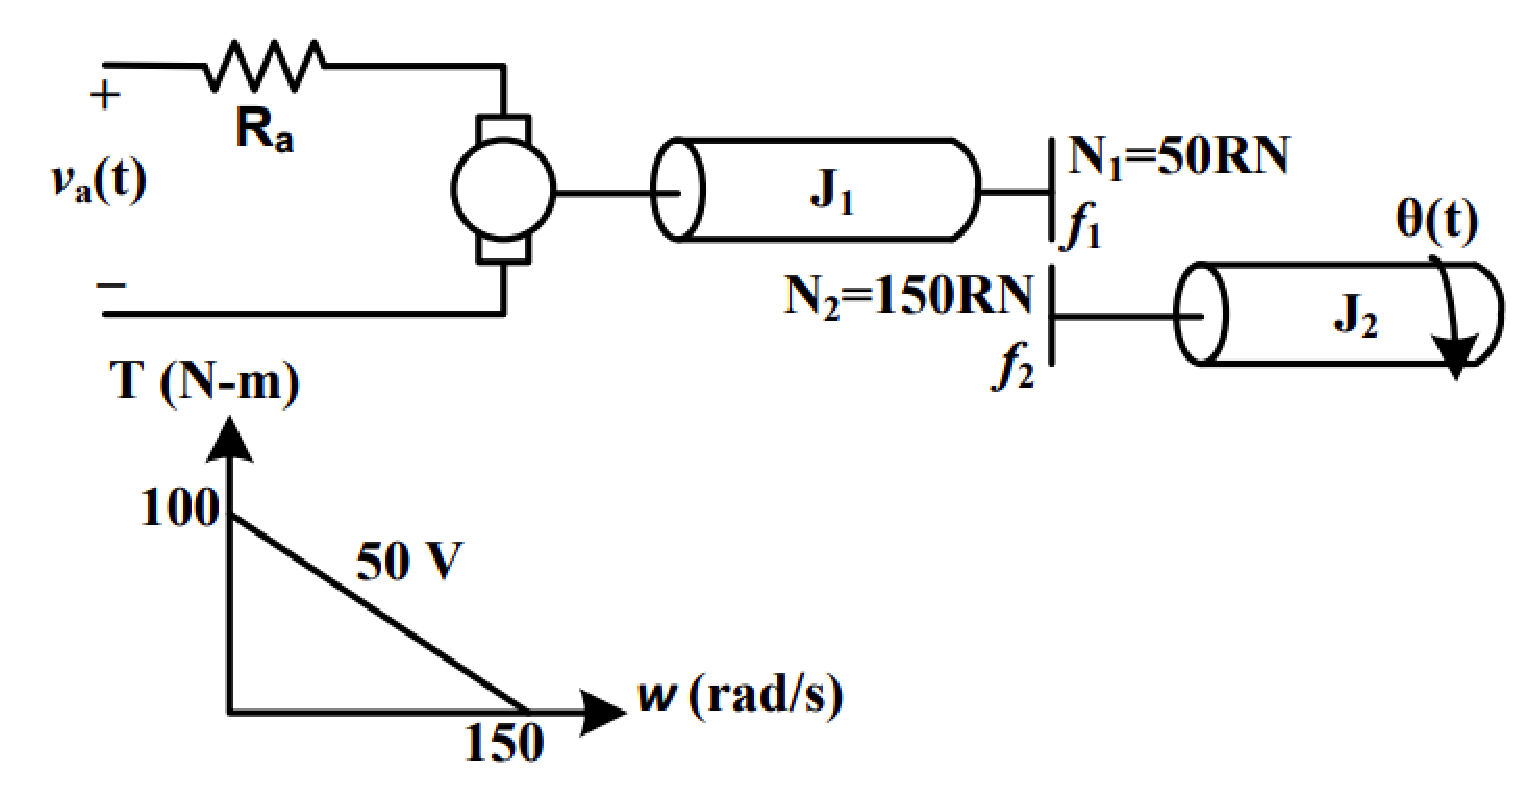
\includegraphics[width=\columnwidth]{./figs/ee18btech11001/ee18btech11001_1.eps}
  \caption{}
  \label{fig:ee18btech11001_fig1}
\end{figure}
%
\solution
Solving the system shown in \ref{fig:ee18btech11001_fig1},

From speed-torque curve of DC Motor in figure. Let $\vec{T_{m}}$ be the torque exerted by DC Motor.  \ref{fig:ee18btech11001_fig1}
\begin{align}
   \vec{T_{m}} &=  \frac{\vec{K_{T}}}{R_{a}}V_{a} - \frac{\vec{K_{T}}.\vec{K_{v}^{T}}}{R_{a}}\bm{\omega_{1}}
   \\
   \vec{T_{m}} &=  2V_{a} - \frac{2}{3}\bm{\omega_{1}}
    \label{eq:ee18btech11001_1}
\end{align}

\begin{table}[!ht]
\centering
\input{./tables/ee18btech11001_3.tex}
\caption{List of Variables}
\label{table:ee18btech11001_3}
\end{table}
Change in torque across ends = torque applied on load + viscous friction. On $J_{1}$ at one end torque $T_{m}$ is applied and at the other end $T_{1}$ exists.
\begin{align}
    \vec{T_{m}} &= \vec{T_{1}} + J_{1}\bm{\Ddot{\theta_{1}}} + f_{1}\bm{\Dot{\theta_{1}}} 
    \label{eq:ee18btech11001_2}
\end{align}
Similarly for $J_{2}$
\begin{align}
    \vec{T_{2}} &=  J_{2}\bm{\Ddot{\theta_{2}}} + f_{2}\bm{\Dot{\theta_{2}}} 
    \label{eq:ee18btech11001_3}
    \\
    \vec{T_{2}} &= \frac{N_{2}}{N_{1}} \vec{T_{1}} \text{ (Gear Train Formula)} \label{eq:ee18btech11001_4}
    \\
    \bm{\theta_{2}} &= \frac{N_{1}}{N_{2}} \bm{\theta_{1}} \text{ (Gear Train Formula)} \label{eq:ee18btech11001_5}
\end{align}

\begin{table}[!ht]
\centering
\input{./tables/ee18btech11001_4.tex}
\caption{Vectors and Matrices}
\label{table:ee18btech11001_4}
\end{table}    
Converting to State Space model
\begin{align}
    \bm{\theta} &= \myvec{\bm{\theta_{1}} \\ \bm{\theta_{2}}}
    \\
    3 \Vec{T_{m}} &= \myvec{3J_{1} & J_{2}}\bm{\Ddot{\theta}}+ \myvec{3f_{1} & f_{2}}\bm{\dot{\theta}}
    \\
    \Vec{T_{m}} &= 2V_{a} - \myvec{\frac{2}{3} & 0}\bm{\dot{\theta}}
    \\
    \bm{\theta} &= \myvec{N_{2} & 0 \\ 0& N_{1}} K
\end{align}
This is the state space model obtained
\begin{align}
    \bm{\Ddot{\theta}} &= \myvec{\frac{-13}{6} & 0 \\ 0 &\frac{-5}{3}}\bm{\Dot{\theta}} + \myvec{\frac{1}{2} \\ \frac{1}{6}}V_{a}
    \\
    \bm{\dot{\theta_{2}}} &= \myvec{0 \\ 1}\bm{\dot{\theta}} 
\end{align}
On solving the above State Space Model
\begin{align}
    V_{a}(s) &= (6s+10)(s\theta_{2}(s)) \label{eq:ee18btech11001_6}
    \\
    G(s) &=  K \frac{\theta (s)}{V_{a}(s)} = \frac{K}{2s(3s+5)} \label{eq:ee18btech11001_7}
\end{align}
From Error Constant  K = 500
\begin{align}
   G(s) &=  \frac{\theta (s)}{V_{a}(s)} = 250 \frac{1}{s(3s+5)} \label{eq:ee18btech11001_8}
   \\
   \zeta &= 0.0695
   \\
   M_{p} &= e^{\dfrac{-\zeta\pi}{\sqrt{1-\zeta^{2}}}} = 81.6\%
\end{align}
\begin{align}
   \phi_{M} &= \tan^{-1}(\dfrac{2\zeta}{\sqrt{-2\zeta^2 + \sqrt{4\zeta^4 + 1}}})
   \\
   \phi_{max} &= 39.5\degree-7.35\degree+ \text{ correction factor}
   \\
   \phi_{max} &= 57\degree
\end{align}
\begin{table}[!ht]
\centering
\begin{enumerate}[label=\thesubsection.\arabic*.,ref=\thesubsection.\theenumi]
\numberwithin{equation}{enumi}
\item A position control system is to be designed such that maximum peak overshoot is less than 25 \%.
Further, appropriate error constant should be 50. For the motor to be used, load and torque
speed curve is shown below, where, $J_{1}$ = 2 kg-m2
, $J_{2}$ = 18 kg-m2
, $f_{1}$ = 2 N-m-s/rad, $f_{2}$ = 36 N-ms/rad. (Although obvious, consider position as the controlled variable and armature voltage as
the manipulated variable.). 
\begin{enumerate}[label=(\roman*)]
\item Design a lead compensator for the system.
\item Design a lag compensator for the system.
\end{enumerate}

\begin{figure}[!ht]
\centering
    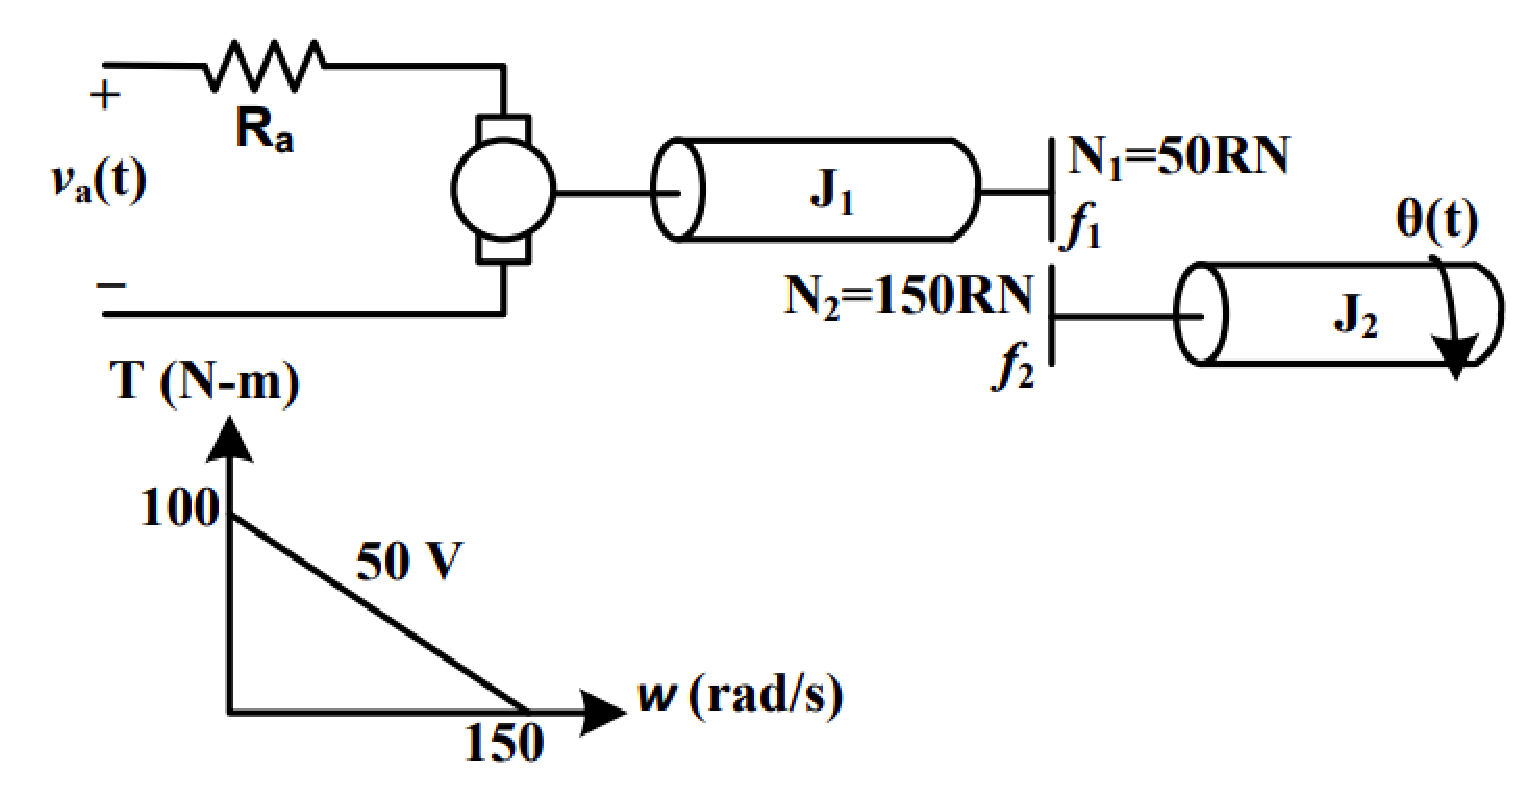
\includegraphics[width=\columnwidth]{./figs/ee18btech11001/ee18btech11001_1.eps}
  \caption{}
  \label{fig:ee18btech11001_fig1}
\end{figure}
%
\solution
Solving the system shown in \ref{fig:ee18btech11001_fig1},

From speed-torque curve of DC Motor in figure. Let $\vec{T_{m}}$ be the torque exerted by DC Motor.  \ref{fig:ee18btech11001_fig1}
\begin{align}
   \vec{T_{m}} &=  \frac{\vec{K_{T}}}{R_{a}}V_{a} - \frac{\vec{K_{T}}.\vec{K_{v}^{T}}}{R_{a}}\bm{\omega_{1}}
   \\
   \vec{T_{m}} &=  2V_{a} - \frac{2}{3}\bm{\omega_{1}}
    \label{eq:ee18btech11001_1}
\end{align}

\begin{table}[!ht]
\centering
\input{./tables/ee18btech11001_3.tex}
\caption{List of Variables}
\label{table:ee18btech11001_3}
\end{table}
Change in torque across ends = torque applied on load + viscous friction. On $J_{1}$ at one end torque $T_{m}$ is applied and at the other end $T_{1}$ exists.
\begin{align}
    \vec{T_{m}} &= \vec{T_{1}} + J_{1}\bm{\Ddot{\theta_{1}}} + f_{1}\bm{\Dot{\theta_{1}}} 
    \label{eq:ee18btech11001_2}
\end{align}
Similarly for $J_{2}$
\begin{align}
    \vec{T_{2}} &=  J_{2}\bm{\Ddot{\theta_{2}}} + f_{2}\bm{\Dot{\theta_{2}}} 
    \label{eq:ee18btech11001_3}
    \\
    \vec{T_{2}} &= \frac{N_{2}}{N_{1}} \vec{T_{1}} \text{ (Gear Train Formula)} \label{eq:ee18btech11001_4}
    \\
    \bm{\theta_{2}} &= \frac{N_{1}}{N_{2}} \bm{\theta_{1}} \text{ (Gear Train Formula)} \label{eq:ee18btech11001_5}
\end{align}

\begin{table}[!ht]
\centering
\input{./tables/ee18btech11001_4.tex}
\caption{Vectors and Matrices}
\label{table:ee18btech11001_4}
\end{table}    
Converting to State Space model
\begin{align}
    \bm{\theta} &= \myvec{\bm{\theta_{1}} \\ \bm{\theta_{2}}}
    \\
    3 \Vec{T_{m}} &= \myvec{3J_{1} & J_{2}}\bm{\Ddot{\theta}}+ \myvec{3f_{1} & f_{2}}\bm{\dot{\theta}}
    \\
    \Vec{T_{m}} &= 2V_{a} - \myvec{\frac{2}{3} & 0}\bm{\dot{\theta}}
    \\
    \bm{\theta} &= \myvec{N_{2} & 0 \\ 0& N_{1}} K
\end{align}
This is the state space model obtained
\begin{align}
    \bm{\Ddot{\theta}} &= \myvec{\frac{-13}{6} & 0 \\ 0 &\frac{-5}{3}}\bm{\Dot{\theta}} + \myvec{\frac{1}{2} \\ \frac{1}{6}}V_{a}
    \\
    \bm{\dot{\theta_{2}}} &= \myvec{0 \\ 1}\bm{\dot{\theta}} 
\end{align}
On solving the above State Space Model
\begin{align}
    V_{a}(s) &= (6s+10)(s\theta_{2}(s)) \label{eq:ee18btech11001_6}
    \\
    G(s) &=  K \frac{\theta (s)}{V_{a}(s)} = \frac{K}{2s(3s+5)} \label{eq:ee18btech11001_7}
\end{align}
From Error Constant  K = 500
\begin{align}
   G(s) &=  \frac{\theta (s)}{V_{a}(s)} = 250 \frac{1}{s(3s+5)} \label{eq:ee18btech11001_8}
   \\
   \zeta &= 0.0695
   \\
   M_{p} &= e^{\dfrac{-\zeta\pi}{\sqrt{1-\zeta^{2}}}} = 81.6\%
\end{align}
\begin{align}
   \phi_{M} &= \tan^{-1}(\dfrac{2\zeta}{\sqrt{-2\zeta^2 + \sqrt{4\zeta^4 + 1}}})
   \\
   \phi_{max} &= 39.5\degree-7.35\degree+ \text{ correction factor}
   \\
   \phi_{max} &= 57\degree
\end{align}
\begin{table}[!ht]
\centering
\input{./tables/ee18btech11001.tex}
\caption{Table of Specifications}
\label{table:ee18btech11001}
\end{table}

\textbf{Designing a lead compensator}
\begin{align}
   G_{c}(s) &=  \frac{1}{a}\frac{s + \frac{1}{T}}{s + \frac{1}{aT}} (a<1) \label{eq:ee18btech11001_9}
   \\
   \sin\phi_{max} &= \dfrac{a-1}{a+1}
   \\
   a &= 0.1
\end{align}
\begin{align}
   |G(j\omega_{c})| &= \frac{1}{\sqrt{a}} = 10 dB
   \\
   \omega_{c} &= 5\degree \text{  (Refer figure \ref{fig:ee18btech11001_fig3})}
   \\
   T &= \frac{1}{\omega_{c}\sqrt{a}} = 0.632
   \\
   G_{c}(s) &=  10 \frac{s + 1.6}{s + 16}
   \\
   G(s)G_{c}(s)  &= 2500 \dfrac{s+1.6}{s(3s+5)(s+16)} \label{eq:ee18btech11001_10}
\end{align}

\textbf{Designing a lag compensator}
\begin{align}
   G_{c}(s) &=  \frac{1}{b}\frac{s + \frac{1}{T}}{s + \frac{1}{bT}} (b>1)  \label{eq:ee18btech11001_11}
   \\
   \phi_{max}  &= 39.5\degree -7.35\degree + correction factor
   \\
   \phi_{max} &= 45 \degree
\end{align}
\begin{figure}[!ht]
\centering
    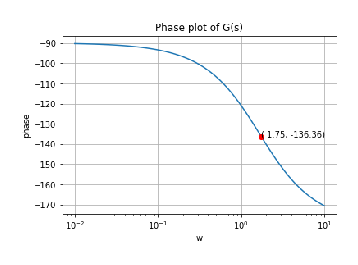
\includegraphics[width=\columnwidth]{./figs/ee18btech11001/ee18btech11001_3.eps}
  \caption{Phase plot of G(s)}
  \label{fig:ee18btech11001_fig2}
\end{figure}

$\omega_{c} = $ Frequency at which phase of bode plot of G(s) is -180 $+ \phi_{max}$ i.e. -135 \degree

$\omega_{c}  = 1.75 rad/sec$  as in Figure \ref{fig:ee18btech11001_fig2}

We place the zero at 
\begin{align} 
   \omega &= 0.2\omega_{c} = 0.35 rad/sec 
   \\
   \implies T &= 2.85
\end{align}
\begin{figure}[!ht]
\centering
    \includegraphics[width=\columnwidth]{./figs/ee18btech11001/ee18btech11001_2.eps}
  \caption{Magnitude plot of G(s)}
  \label{fig:ee18btech11001_fig3}
\end{figure}
\begin{lstlisting}
codes/ee18btech11001/ee18btech11001_1.py
\end{lstlisting}

The magnitude of $G(j\omega)$ at the new gain crossover frequency  $\omega_{c} = 1.75 rad/sec$ is 26 dB as in figure \ref{fig:ee18btech11001_fig3}.In order to have $\omega_{c}$  as the new gain crossover frequency, the lag compensator
must give an attenuation of -26db at $\omega_{c}$
\begin{align}
    -20 \log{b} &= -26dB
    \\
    b &= 19.95 \approx 20
    \\
    G_{c}(s) &=  0.05\frac{s + 0.35}{s + 0.0175}
    \\
    G(s)G_{c}(s) &= 12.5 \dfrac{s+0.35}{s(3s+5)(s+0.0175)} \label{eq:ee18btech11001_12}
\end{align}


\textbf{Performance Evaluation of compensators}

The following code plots the performance curves

\begin{lstlisting}[frame=single]
codes/ee18btech11001/ee18btech11001_2.py
\end{lstlisting}
\begin{figure}[!ht]
\centering
    \includegraphics[width=\columnwidth]{./figs/ee18btech11001/ee18btech11001_4.eps}
  \caption{Performance of Lead Compensator}
  \label{fig:ee18btech11001_fig4}
\end{figure}
\begin{figure}[!ht]
\centering
    \includegraphics[width=\columnwidth]{./figs/ee18btech11001/ee18btech11001_5.eps}
  \caption{Performance of Lag Compensator}
  \label{fig:ee18btech11001_fig5}
\end{figure}

\begin{table}[!ht]
\centering
\input{./tables/ee18btech11001_2.tex}
\caption{Performance comparison}
\label{table:ee18btech11001_2}
\end{table}
Figures \ref{fig:ee18btech11001_fig4} and \ref{fig:ee18btech11001_fig5} show the reduced overshoot \& settling time for unit step input. 

\textbf{\newline This verifies that the designed lead and lag compensators work as per specifications.} 
\end{enumerate}

\caption{Table of Specifications}
\label{table:ee18btech11001}
\end{table}

\textbf{Designing a lead compensator}
\begin{align}
   G_{c}(s) &=  \frac{1}{a}\frac{s + \frac{1}{T}}{s + \frac{1}{aT}} (a<1) \label{eq:ee18btech11001_9}
   \\
   \sin\phi_{max} &= \dfrac{a-1}{a+1}
   \\
   a &= 0.1
\end{align}
\begin{align}
   |G(j\omega_{c})| &= \frac{1}{\sqrt{a}} = 10 dB
   \\
   \omega_{c} &= 5\degree \text{  (Refer figure \ref{fig:ee18btech11001_fig3})}
   \\
   T &= \frac{1}{\omega_{c}\sqrt{a}} = 0.632
   \\
   G_{c}(s) &=  10 \frac{s + 1.6}{s + 16}
   \\
   G(s)G_{c}(s)  &= 2500 \dfrac{s+1.6}{s(3s+5)(s+16)} \label{eq:ee18btech11001_10}
\end{align}

\textbf{Designing a lag compensator}
\begin{align}
   G_{c}(s) &=  \frac{1}{b}\frac{s + \frac{1}{T}}{s + \frac{1}{bT}} (b>1)  \label{eq:ee18btech11001_11}
   \\
   \phi_{max}  &= 39.5\degree -7.35\degree + correction factor
   \\
   \phi_{max} &= 45 \degree
\end{align}
\begin{figure}[!ht]
\centering
    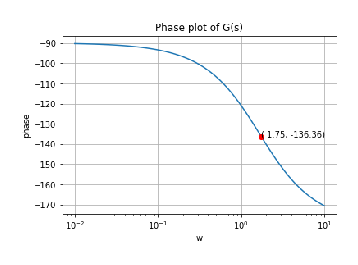
\includegraphics[width=\columnwidth]{./figs/ee18btech11001/ee18btech11001_3.eps}
  \caption{Phase plot of G(s)}
  \label{fig:ee18btech11001_fig2}
\end{figure}

$\omega_{c} = $ Frequency at which phase of bode plot of G(s) is -180 $+ \phi_{max}$ i.e. -135 \degree

$\omega_{c}  = 1.75 rad/sec$  as in Figure \ref{fig:ee18btech11001_fig2}

We place the zero at 
\begin{align} 
   \omega &= 0.2\omega_{c} = 0.35 rad/sec 
   \\
   \implies T &= 2.85
\end{align}
\begin{figure}[!ht]
\centering
    \includegraphics[width=\columnwidth]{./figs/ee18btech11001/ee18btech11001_2.eps}
  \caption{Magnitude plot of G(s)}
  \label{fig:ee18btech11001_fig3}
\end{figure}
\begin{lstlisting}
codes/ee18btech11001/ee18btech11001_1.py
\end{lstlisting}

The magnitude of $G(j\omega)$ at the new gain crossover frequency  $\omega_{c} = 1.75 rad/sec$ is 26 dB as in figure \ref{fig:ee18btech11001_fig3}.In order to have $\omega_{c}$  as the new gain crossover frequency, the lag compensator
must give an attenuation of -26db at $\omega_{c}$
\begin{align}
    -20 \log{b} &= -26dB
    \\
    b &= 19.95 \approx 20
    \\
    G_{c}(s) &=  0.05\frac{s + 0.35}{s + 0.0175}
    \\
    G(s)G_{c}(s) &= 12.5 \dfrac{s+0.35}{s(3s+5)(s+0.0175)} \label{eq:ee18btech11001_12}
\end{align}


\textbf{Performance Evaluation of compensators}

The following code plots the performance curves

\begin{lstlisting}[frame=single]
codes/ee18btech11001/ee18btech11001_2.py
\end{lstlisting}
\begin{figure}[!ht]
\centering
    \includegraphics[width=\columnwidth]{./figs/ee18btech11001/ee18btech11001_4.eps}
  \caption{Performance of Lead Compensator}
  \label{fig:ee18btech11001_fig4}
\end{figure}
\begin{figure}[!ht]
\centering
    \includegraphics[width=\columnwidth]{./figs/ee18btech11001/ee18btech11001_5.eps}
  \caption{Performance of Lag Compensator}
  \label{fig:ee18btech11001_fig5}
\end{figure}

\begin{table}[!ht]
\centering
\input{./tables/ee18btech11001_2.tex}
\caption{Performance comparison}
\label{table:ee18btech11001_2}
\end{table}
Figures \ref{fig:ee18btech11001_fig4} and \ref{fig:ee18btech11001_fig5} show the reduced overshoot \& settling time for unit step input. 

\textbf{\newline This verifies that the designed lead and lag compensators work as per specifications.} 
\end{enumerate}

\caption{Table of Specifications}
\label{table:ee18btech11001}
\end{table}

\textbf{Designing a lead compensator}
\begin{align}
   G_{c}(s) &=  \frac{1}{a}\frac{s + \frac{1}{T}}{s + \frac{1}{aT}} (a<1) \label{eq:ee18btech11001_9}
   \\
   \sin\phi_{max} &= \dfrac{a-1}{a+1}
   \\
   a &= 0.1
\end{align}
\begin{align}
   |G(j\omega_{c})| &= \frac{1}{\sqrt{a}} = 10 dB
   \\
   \omega_{c} &= 5\degree \text{  (Refer figure \ref{fig:ee18btech11001_fig3})}
   \\
   T &= \frac{1}{\omega_{c}\sqrt{a}} = 0.632
   \\
   G_{c}(s) &=  10 \frac{s + 1.6}{s + 16}
   \\
   G(s)G_{c}(s)  &= 2500 \dfrac{s+1.6}{s(3s+5)(s+16)} \label{eq:ee18btech11001_10}
\end{align}

\textbf{Designing a lag compensator}
\begin{align}
   G_{c}(s) &=  \frac{1}{b}\frac{s + \frac{1}{T}}{s + \frac{1}{bT}} (b>1)  \label{eq:ee18btech11001_11}
   \\
   \phi_{max}  &= 39.5\degree -7.35\degree + correction factor
   \\
   \phi_{max} &= 45 \degree
\end{align}
\begin{figure}[!ht]
\centering
    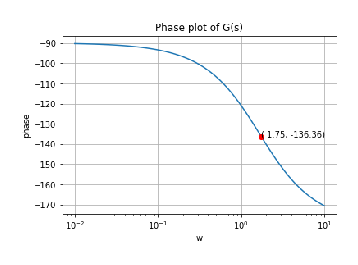
\includegraphics[width=\columnwidth]{./figs/ee18btech11001/ee18btech11001_3.eps}
  \caption{Phase plot of G(s)}
  \label{fig:ee18btech11001_fig2}
\end{figure}

$\omega_{c} = $ Frequency at which phase of bode plot of G(s) is -180 $+ \phi_{max}$ i.e. -135 \degree

$\omega_{c}  = 1.75 rad/sec$  as in Figure \ref{fig:ee18btech11001_fig2}

We place the zero at 
\begin{align} 
   \omega &= 0.2\omega_{c} = 0.35 rad/sec 
   \\
   \implies T &= 2.85
\end{align}
\begin{figure}[!ht]
\centering
    \includegraphics[width=\columnwidth]{./figs/ee18btech11001/ee18btech11001_2.eps}
  \caption{Magnitude plot of G(s)}
  \label{fig:ee18btech11001_fig3}
\end{figure}
\begin{lstlisting}
codes/ee18btech11001/ee18btech11001_1.py
\end{lstlisting}

The magnitude of $G(j\omega)$ at the new gain crossover frequency  $\omega_{c} = 1.75 rad/sec$ is 26 dB as in figure \ref{fig:ee18btech11001_fig3}.In order to have $\omega_{c}$  as the new gain crossover frequency, the lag compensator
must give an attenuation of -26db at $\omega_{c}$
\begin{align}
    -20 \log{b} &= -26dB
    \\
    b &= 19.95 \approx 20
    \\
    G_{c}(s) &=  0.05\frac{s + 0.35}{s + 0.0175}
    \\
    G(s)G_{c}(s) &= 12.5 \dfrac{s+0.35}{s(3s+5)(s+0.0175)} \label{eq:ee18btech11001_12}
\end{align}


\textbf{Performance Evaluation of compensators}

The following code plots the performance curves

\begin{lstlisting}[frame=single]
codes/ee18btech11001/ee18btech11001_2.py
\end{lstlisting}
\begin{figure}[!ht]
\centering
    \includegraphics[width=\columnwidth]{./figs/ee18btech11001/ee18btech11001_4.eps}
  \caption{Performance of Lead Compensator}
  \label{fig:ee18btech11001_fig4}
\end{figure}
\begin{figure}[!ht]
\centering
    \includegraphics[width=\columnwidth]{./figs/ee18btech11001/ee18btech11001_5.eps}
  \caption{Performance of Lag Compensator}
  \label{fig:ee18btech11001_fig5}
\end{figure}

\begin{table}[!ht]
\centering
\input{./tables/ee18btech11001_2.tex}
\caption{Performance comparison}
\label{table:ee18btech11001_2}
\end{table}
Figures \ref{fig:ee18btech11001_fig4} and \ref{fig:ee18btech11001_fig5} show the reduced overshoot \& settling time for unit step input. 

\textbf{\newline This verifies that the designed lead and lag compensators work as per specifications.} 
\end{enumerate}

\caption{}
\label{table:ee18btech11001}
\end{table}


%-----------------------------------------------------------------------%

\item Obtain the transfer function of $H(s)$.
\\
\solution From Table \ref{table:ee18btech11001},
{\footnotesize
\begin{align}
\label{eq:ee18btech11001_system}
	H(s) = \frac{K(s+j2\pi 10^{3})(s+j2\pi 10^{4})^{2}}{(s+j2\pi 10^{1})(s+j2\pi 10^{2})^{2}(s+j2\pi 10^{5})^{2}(s+j2\pi 10^{6})}
\end{align}
}
\item Justify the above results.
\\
\solution
Let us consider a generalized transfer gain
\begin{align}
	H(s) = k \dfrac{(s-z_{1})(s-z_{2})...(s-z_{m-1})(s-z_{m})}{(s-p_{1})(s-p_{2})....(s-p_{n-1})(s-p_{n})}
\end{align}
The gain
\begin{multline}
	G(f) = 20\log\abs{H(s)} 
\\
= 20\log \abs{k} + 20\log \abs{s-z_{1}} 
	    \\
	    + 20\log \abs{s-z_{2}} + \dots + 20\log \abs{s-z_{m}} 
\\
- 20\log \abs{s-p_{1}} 
	    - 20\log \abs{s-p_{2}} 
	    \\
- \dots - 20\log \abs{s-z_{n}} 
\end{multline}
%
Substituting $s = \j \omega$, for real $z_1$
\begin{align}
	20\log \abs{s-z_{1}} &= 20\log \abs{\sqrt{\omega^{2} + z_{1}^{2}}}
\\
&= 
\begin{cases}
20 \log \abs{z_{1}}, & \omega \ll z_{1}
\\
20 \log \abs{\omega}, & \omega \gg z_{1}
\end{cases}
\end{align}
%
Taking the derivative, 
\begin{align}
	\frac{d\brak{20\log \abs{s-z_{1}}}}{d\brak{\log \abs{\omega}}} 
= 
\begin{cases}
0, & \omega \ll z_{1}
\\
20, & \omega \gg z_{1}
\end{cases}
\end{align}
%
Thus, when a zero is encountered, the gradient of $H(\j\omega)$ jumps by +20 in the log scale.  When a pole is encountered, the gradient falls by -20. Note that this is a very loose justification, but works well in practice.

%-----------------------------------------------------------------------%

\item Obtain the Bode plot and the slope plot for $H(s)$ and verify with  Fig. \ref{fig:ee18btech11001_bode}
\\
\solution Bode Plot of obtained Transfer Function is 
\begin{figure}[htp]
    \centering
    \includegraphics[width=\columnwidth]{./figs/ee18btech11001/ee18btech11001_2.eps}
    \caption{}
    \label{fig:ee18btech11001_2}
\end{figure}
%
Fig. \ref{fig:ee18btech11001}, obtained from  \eqref{eq:ee18btech11001_system},
is a close reconstruction of Fig. \ref{fig:ee18btech11001}.
\end{enumerate}


